% !TeX root = ../main.tex

\chapter{MẠNG NƠ-RON TÍCH CHẬP VÀ MÔ HÌNH YOLO}

\section{Bài toán phát hiện vật thể}

Phát hiện vật thể là một bài toán quan trọng trong thị giác máy tính với mục tiêu xác định vị trí và loại vật thể trong ảnh. Đầu vào của bài toán phát hiện vật thể thường là ảnh hoặc từng khung hình trong băng hình, đầu ra là các hộp bao xác định vị trí, kích thước của đối tượng và nhãn xác định loại đối tượng.

Các loại vật thể trong bài toán này có thể bao gồm người, xe cộ, động vật hay đồ vật thường ngày, v.v. Vì vậy, ứng dụng của bài toán phát hiện vật thể cũng rất đa dạng:
\begin{itemize}
	\item Nhận diện, theo dõi đối tượng trong an ninh, giám sát.
	\item Tự động lái và hỗ trợ lái xe, phát hiện người, xe, vật cản, v.v.
	\item Phân tích hành vi người dùng qua hình ảnh.
	\item Phát hiện các sự cố, rủi ro trong nhà máy, công nghiệp.
	\item Phát hiện và nhận diện vật dụng hỗ trợ người khuyết tật.
	\item Phát hiện trạng thái sinh trưởng, tình trạng sức khỏe cây trồng trong nông nghiệp.
\end{itemize}

Bài toán phát hiện vật thể có thể thực hiện sử dụng hai phương pháp, phương pháp phát hiện vật thể một bước và phương pháp phát hiện vật thể hai bước\cite{kang2022}:
\begin{itemize}
	\item Phương pháp phát hiện vật thể một bước: là phương pháp triển khai mô hình \acrshort{cnn} trong đó toàn bộ quá trình phát hiện vật thể được thực hiện trong một bước duy nhất. Các mạng trong nhóm này thường sử dụng các mô hình \acrshort{cnn} để trực tiếp dự đoán các hộp bao và các lớp của các vật thể trong một hình ảnh.	Một số ví dụ nổi bật của phương pháp này bao gồm: \acrshort{yolo}, SSD.
	
	\item Phương pháp phát hiện vật thể hai bước: là phương pháp phát hiện vật thể đầu tiên sử dụng \acrshort{cnn} theo 2 bước: Tạo các đề xuất vùng có khả năng cao chứa đối tượng và giai đoạn phân loại từng vùng được đề xuất, tinh chỉnh tọa độ hộp bao. Các thuật toán sử dụng phương pháp này bao gồm R-\acrshort{cnn}, Fast R-\acrshort{cnn} hay Faster R-\acrshort{cnn}.
\end{itemize}

Về tốc độ, phương pháp một bước thường nhanh hơn, phù hợp với các ứng dụng thời gian thực.

Về độ chính xác, phương pháp hai bước có độ chính xác cao hơn, đặc biệt là trong việc phát hiện các vật thể nhỏ hoặc trong các hình ảnh phức tạp. Phương pháp một bước có kém chính xác hơn nhưng đang dần được cải thiện trong các phiên bản mới hơn.

Về độ phức tạp, phương pháp hai bước phức tạp hơn trong triển khai và yêu cầu tài nguyên tính toán lớn hơn. Phương pháp một bước đơn giản hơn và dễ dàng triển khai trong các ứng dụng thực tế và các thiết bị nhúng.


\section{Mạng nơ-ron tích chập}

\subsection{Mạng nơ-ron}

Mạng nơ-ron là một hệ thống của các nơ-ron nhân tạo được kết nối với nhau và trao đổi thông điệp qua lại. Các kết nối này có trọng số số học được điều chỉnh trong quá trình huấn luyện, để một mạng được huấn luyện đúng cách sẽ phản hồi chính xác khi được trình bày với một hình ảnh hoặc mẫu để nhận dạng. Mạng bao gồm nhiều lớp của các “nơ-ron” phát hiện đặc trưng. Mỗi lớp có nhiều nơ-ron phản ứng với các tổ hợp khác nhau của các đầu vào từ các lớp trước đó. Như được minh họa trong hình \ref{fig:ann-intro}, các lớp được xây dựng để lớp đầu tiên phát hiện một tập hợp các mẫu nguyên thủy trong đầu vào, lớp thứ hai phát hiện các mẫu của các mẫu, lớp thứ ba phát hiện các mẫu của những mẫu đó, và cứ tiếp tục như vậy. Các mạng điển hình sử dụng từ 5 đến 25 lớp khác biệt để nhận dạng mẫu.
\begin{figure}[h]
	\centering
	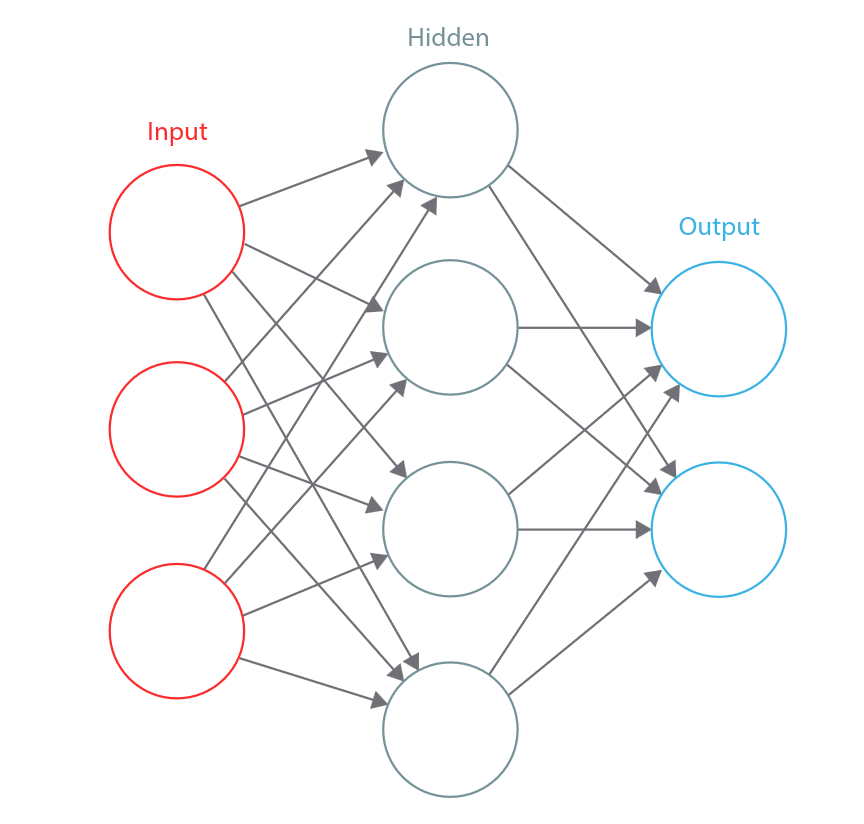
\includegraphics[width=0.6\linewidth]{images/ann-intro}
	\caption{Mạng nơ-ron nhân tạo\cite{hijazi2015UsingCN}}
	\label{fig:ann-intro}
\end{figure}

Hình \ref{fig:math-ann} mô tả mô hình toán học của một nơ-ron, mỗi nơ-ron nhận các tham số đầu vào $x_0, x_1, x_2, ..., x_n$, nhân mỗi tham số đầu vào với từng trọng số $w_0, w_1, w_2, ..., w_n$, lấy tổng cùng với độ lệch $b$ để thu được kết quả đầu ra.

\begin{figure}[H]
	\centering
	\begin{subfigure}{.5\textwidth}
		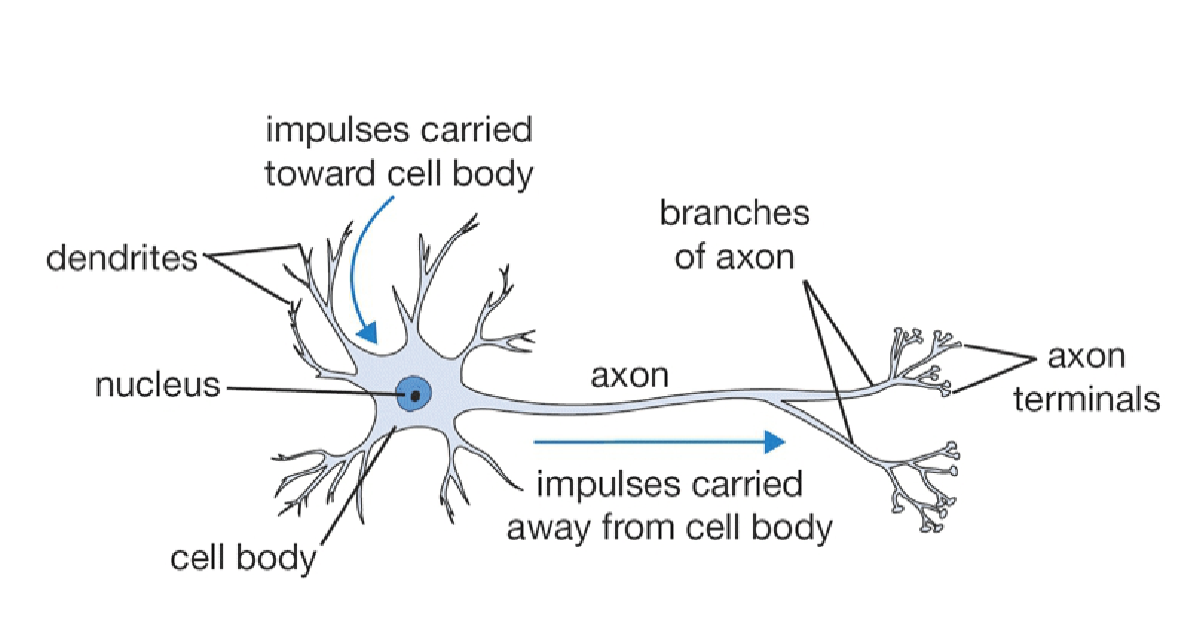
\includegraphics[width=0.9\linewidth]{images/real-neural.png}
	\end{subfigure}%
	\begin{subfigure}{.5\textwidth}
		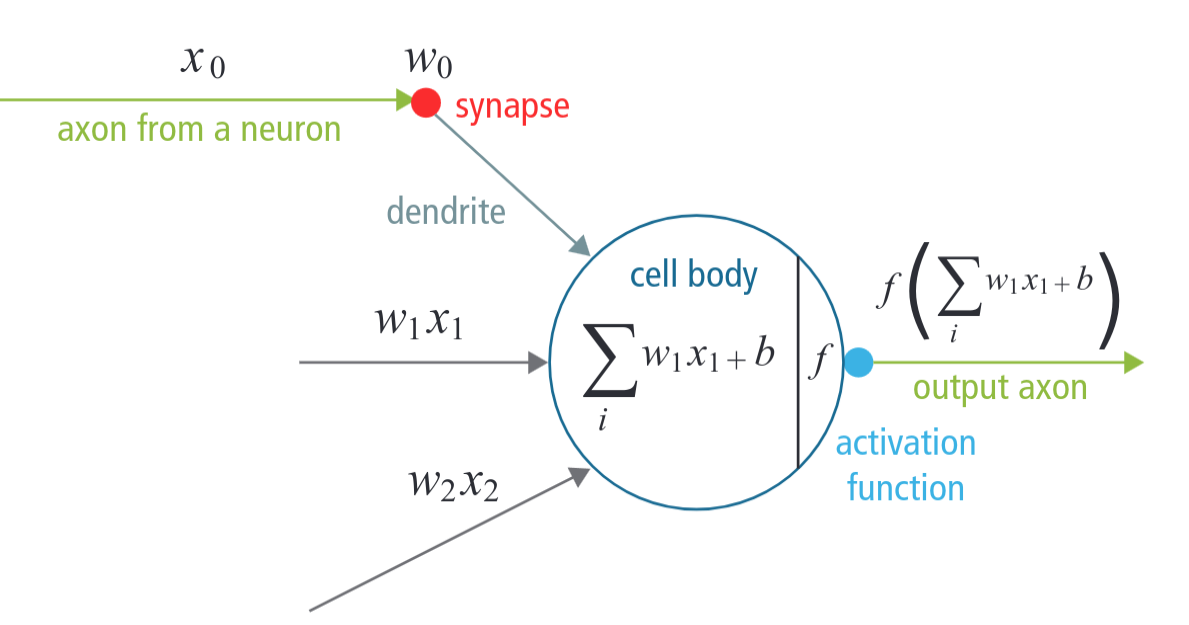
\includegraphics[width=0.9\linewidth]{images/artificial-neural.png}
	\end{subfigure}
	\caption{Mô phỏng một nơ-ron bằng mô hình toán học \cite{karpathy}}
	\label{fig:math-ann}
\end{figure}

Trong quá trình huấn luyện mạng nơ-ron, các mẫu với nhãn tương ứng được đưa vào mạng để tinh chỉnh các giá trị trọng số $w$ và độ lệch $b$ như hình \ref{fig:artificial-neural-training}.

\begin{figure}[h]
	\centering
	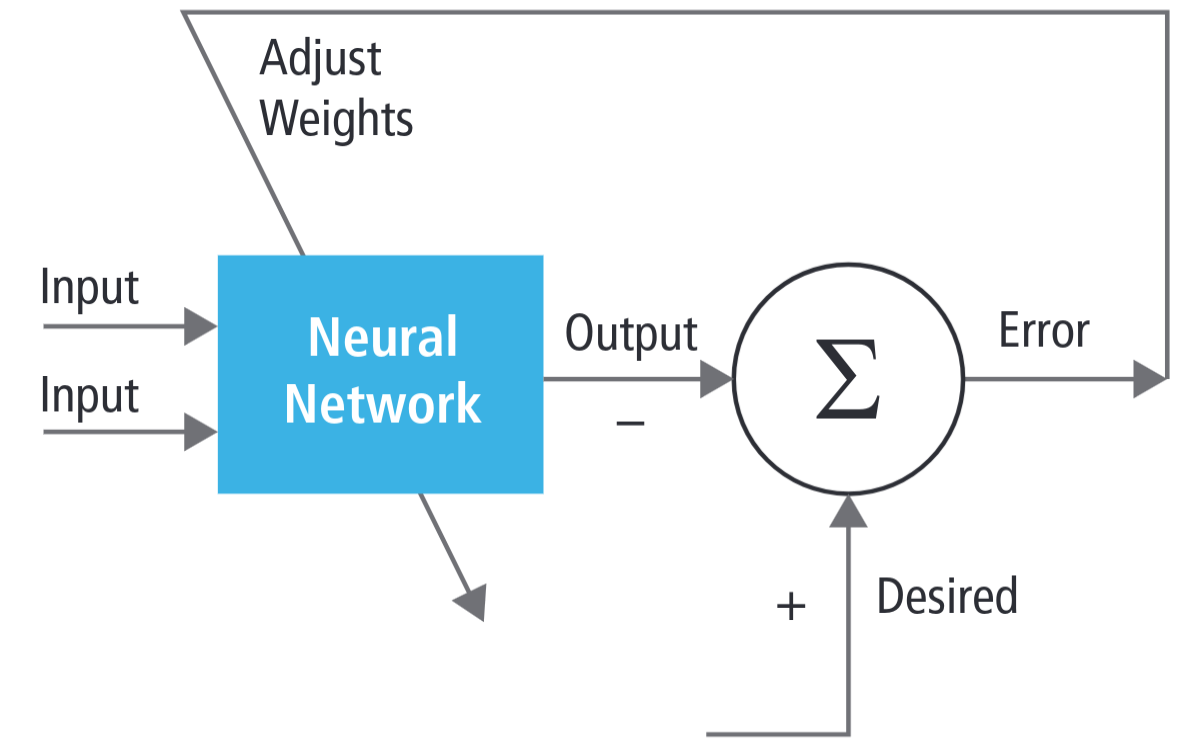
\includegraphics[width=0.5\linewidth]{images/artificial-neural-training}
	\caption{Quá trình huấn luyện mạng nơ-ron nhân tạo}
	\label{fig:artificial-neural-training}
\end{figure}



\subsection{Giới thiệu mạng nơ-ron tích chập}

Với đầu vào là ảnh, việc xử lý sử dụng mạng nơ-ron nhân tạo yêu cầu làm "phẳng" dữ liệu thành một véc-tơ đầu vào. Điều này làm chậm quá trình tính toán, yêu cầu dữ liệu đầu vào phù hợp với kích thước của mạng và tăng lượng bộ nhớ yêu cầu cho việc tính toán. Do trong dạng dữ liệu ảnh, các điểm ảnh cạnh nhau có quan hệ mật thiết, việc tính toán có thể được giảm nhờ vào việc giảm kích thước của ảnh nhờ các phép tích chập. Vì vậy, \acrshort{cnn} là một dạng của mạng nơ-ron \cite{oshea2015introduction} được sử dụng phổ biến trong lĩnh vực xử lý ảnh và nhận dạng đối tượng.

Đặc điểm chính của \acrshort{cnn} bao gồm:

\begin{itemize}
	\item Lớp tích chập: là lớp cốt lõi của \acrshort{cnn}, sử dụng phép tích chập để trích xuất đặc trưng từ ảnh đầu vào. Lớp này sử dụng các bộ lọc để thực hiện phép tích chập trên ảnh và tạo ra các biểu đồ đặc trưng, trong đó mỗi điểm ảnh của biểu đồ đặc trưng biểu diễn mức độ kích hoạt của một đặc trưng cụ thể.
	
	\item Lớp gộp: được sử dụng để giảm kích thước của bản đồ đặc trưng và giảm số lượng tham số trong mạng. Lớp gộp thường áp dụng các phép tổng hợp như lấy giá trị lớn nhất hoặc lấy giá trị trung bình trong một vùng nhất định trên biểu đồ đặc trưng.
	
	\item Lớp kích hoạt: áp dụng một hàm kích hoạt phi tuyến sau lớp tích chập để tạo độ không tuyến tính và giúp mô hình học được các đặc trưng phức tạp hơn.
	
	\item Lớp kết nối đầy đủ: là một loại lớp nơ-ron truyền thống, kết nối các đặc trưng đã được trích xuất từ lớp trước với các nơ ron trong lớp này. Lớp này có thể loại bỏ thường xuất ra các đầu ra cuối cùng của mạng, thường là các xác suất phân loại của các lớp đối tượng.
	
	\item Hàm mất mát: được sử dụng để đánh giá sự khác biệt giữa kết quả dự đoán và giá trị thực tế. Các hàm mất mát phổ biến trong \acrshort{cnn} bao gồm hàm Cross-Entropy và hàm Mean Squared Error.
	
	\item Tính chia sẻ tham số: \acrshort{cnn} sử dụng cơ chế chia sẻ tham số giữa các vùng không gian trong ảnh để giảm số lượng tham số cần học. Thay vì học các trọng số riêng cho mỗi vùng của ảnh, \acrshort{cnn} chia sẻ các trọng số giữa các vùng có cùng đặc trưng.
	
	\item Kiến trúc kiểu "tầng": \acrshort{cnn} được tổ chức thành một chuỗi các lớp xếp chồng lên nhau, mỗi lớp đóng vai trò trong việc trích xuất và học các đặc trưng từ dữ liệu. Kiến trúc kiểu "tầng" giúp mạng học được các đặc trưng từ cấp thấp đến cấp cao, từ các nét cơ bản đến các đặc trưng phức tạp hơn.
\end{itemize}

\begin{figure}
	\centering
	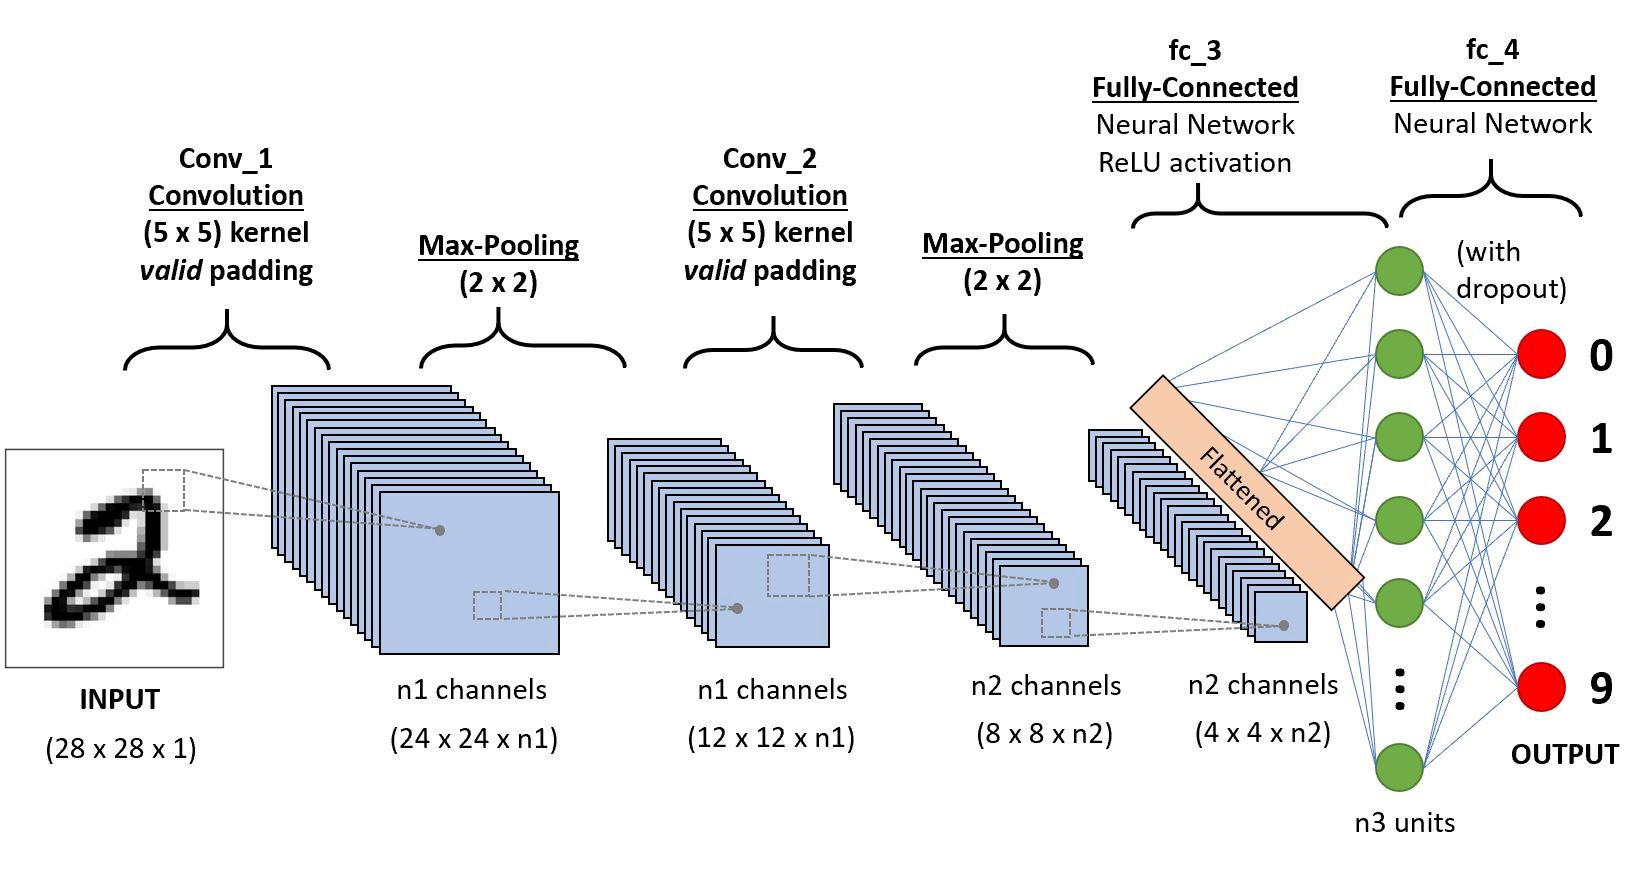
\includegraphics[width=0.9\linewidth]{images/typical-cnn.png}
	\caption{\acrshort{cnn} phát hiện chữ viết tay\cite{ratan_2023}}
	\label{fig:typical-cnn}
\end{figure}

Tổng quan, \acrshort{cnn} là một kiến trúc mạng nơ ron đặc biệt được thiết kế để xử lý và trích xuất đặc trưng từ dữ liệu ảnh. Các đặc điểm của \acrshort{cnn} như lớp tích chập, lớp gộp, lớp kích hoạt, lớp kết nối đầy đủ và tính chia sẻ tham số giúp cho \acrshort{cnn} có khả năng học và trích xuất các đặc trưng từ dữ liệu ảnh một cách hiệu quả. Kiến trúc kiểu "tầng" trong \acrshort{cnn} cho phép mạng học được các đặc trưng từ cấp thấp đến cấp cao, từ các nét cơ bản đến các đặc trưng phức tạp hơn.

\subsection{Cấu trúc mạng nơ-ron tích chập}
\subsubsection{Lớp tích chập}

\textbf{Dữ liệu đầu vào}

Dữ liệu hình ảnh đầu vào cho \acrshort{cnn} thường là các bức ảnh được biểu diễn dưới dạng ma trận điểm ảnh. Mỗi điểm ảnh trong ma trận thể hiện mức độ sáng tại mỗi vị trí trên ảnh.

Thông thường các ảnh màu đầu vào sẽ có các kênh màu RGB, trong đó mỗi kênh màu tương ứng với một thành phần màu đỏ (R), xanh lá cây (G) và xanh dương (B). Với mỗi điểm ảnh, giá trị của từng kênh màu (R, G, B) thường được biểu diễn bằng một con số trong khoảng từ 0 đến 255.

Kích thước của ảnh đầu vào có thể khác nhau tùy thuộc vào yêu cầu của bài toán và kiến trúc của \acrshort{cnn}. Các kích thước phổ biến cho ảnh đầu vào là 224x224, 256x256, 299x299 hoặc 512x512 điểm ảnh.

Trước khi đưa dữ liệu hình ảnh vào \acrshort{cnn}, dữ liệu cần đưa qua một số bước tiền xử lý:

\begin{itemize}
	\item Chuẩn hóa: để đảm bảo rằng các giá trị pixel trong ảnh nằm trong khoảng từ 0 đến 1. Như vậy cần phải chuẩn hóa dữ liệu bằng cách chia tất cả các giá trị điểm ảnh cho 255 đối với kiểu dữ liệu 8 bit hoặc chia cho $2^n-1$ với $n$ là số bit biểu diễn số nguyên của điểm ảnh.
	\item Thay đổi kích thước: nếu kích thước của ảnh không phù hợp với kích thước đầu vào của \acrshort{cnn}, cần thực hiện điều chỉnh kích thước ảnh để phù hợp. Thông thường, sử dụng phép thay đổi tuyến tính hoặc cắt ảnh để thay đổi kích thước ảnh.
	\item Tăng cường dữ liệu huấn luyện: đối với các bài toán sử dụng \acrshort{cnn}, việc sử dụng kỹ thuật tăng cường dữ liệu khi huấn luyện có thể giúp tăng tính tổng quát hóa của mô hình. Tăng cường dữ liệu bao gồm việc áp dụng các phép biến đổi như xoay, lật, phóng to, thu nhỏ, và thay đổi độ sáng để tạo ra các phiên bản mới của dữ liệu hình ảnh.
\end{itemize}

Dữ liệu trong \acrshort{cnn} được biểu diễn dưới dạng ma trận. Dữ liệu hình ảnh đầu vào sẽ được biểu diễn dưới dạng \ref{input_shape}.

\begin{equation}
	\centering
	\label{input_shape}
	(N \times C \times H_{in} \times W_{in})
\end{equation}

Trong đó
\begin{itemize}
	\item $N$ là số hình ảnh đầu vào theo lô.
	\item $C$ là số kênh, ảnh mức xám có số kênh bằng 1, ảnh RGB có số kênh bằng 3.
	\item $H_{in}$ là chiều cao ảnh.
	\item $W_{in}$ là chiều rộng ảnh.
\end{itemize}

\textbf{Phép chập}

Phép chập là một phép toán cơ bản trong xử lý ảnh dùng để xác định đặc trưng giữa các điểm ảnh trong một hình ảnh và xây dựng các bộ lọc để trích xuất đặc trưng hay thực hiện các phép biến đổi hình ảnh. Hình \ref{fig:edge-detection-conv} mô tả ứng dụng của phép tích chập trong bài toán phát hiện biên theo chiều dọc.

% TODO: \usepackage{graphicx} required
\begin{figure}[h]
	\centering
	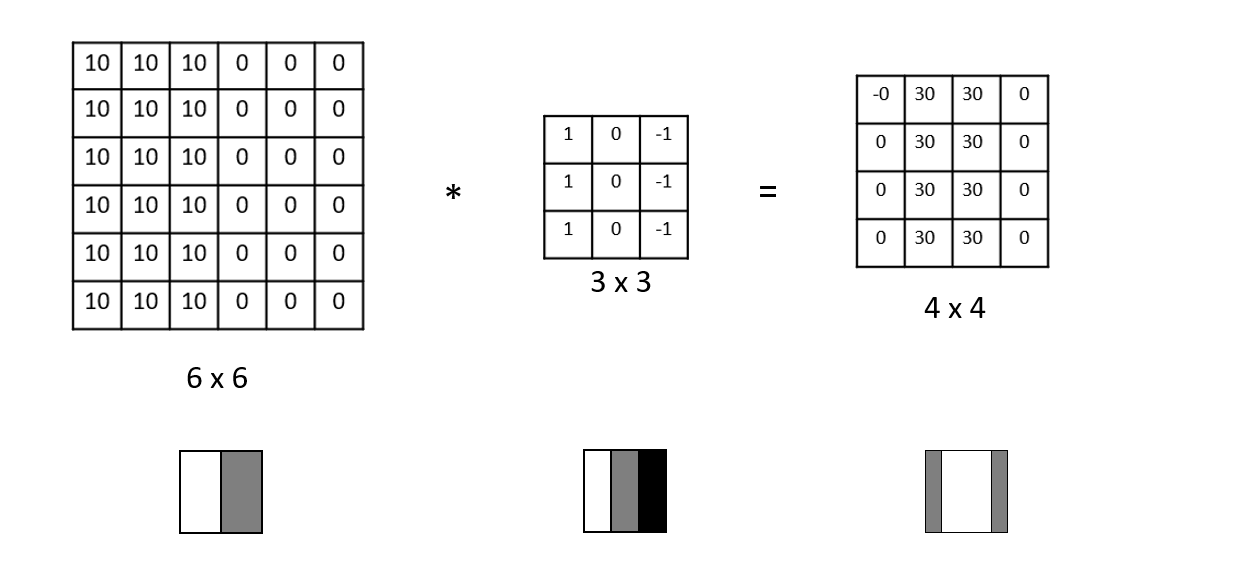
\includegraphics[width=0.8\linewidth]{images/edge-detection-conv}
	\caption{Phép tích chập trong phát hiện dọc}
	\label{fig:edge-detection-conv}
\end{figure}

Bộ lọc hay nhân trong phép tích chập là một ma trận được xoay $180^\circ$, trượt tới từng vị trí của ma trận vào. Kết quả từng vị trí của ma trận kết quả trong phép tích chập tính bằng cách tính tổng của tích từng phần tử của nhân đã được xoay $180^\circ$ với phần tử tại vị trí tương ứng trên ma trận vào. Nói cách khác, kết quả phép chập là kết quả phép tương quan chéo giữa ma trận đầu vào với nhân được xoay $180^\circ$ \ref{eqn:conv-basic}.

\begin{equation}\label{eqn:conv-basic}
	x_{ij} = \sum^{m-1}_{a = 0} \sum^{m-1}_{b = 0} k_{ab} y_{(i+a)(j+b)}, k' = rot180(k)
\end{equation}

Trong thực thế, lớp tích chập trong \acrshort{cnn} có thể loại bỏ phép xoay và sử dụng phép tương quan chéo nhằm mục đích tối ưu tính toán mà không ảnh hưởng tới kết quả của mạng \cite{jorda}. Như vậy, thay vì công thức \ref{eqn:conv-basic} lớp tích chập có thể sử dụng công thức \ref{eqn:correlate-basic} thay thế.

\begin{equation}\label{eqn:correlate-basic}
	x_{ij} = \sum^{m-1}_{a = 0} \sum^{m-1}_{b = 0} k_{ab} y_{(i+a)(j+b)}
\end{equation}

Hình \ref{fig:conv-operation} mô tả quá trình thực hiện chập ma trận vào với bộ lọc để được kết quả phần tử đầu tiên của ma trận ra.

% TODO: \usepackage{graphicx} required
\begin{figure}
	\centering
	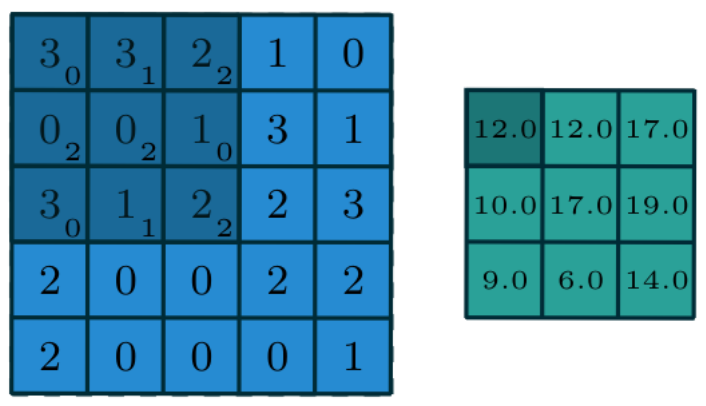
\includegraphics[width=0.6\linewidth]{images/conv-operation}
	\caption{Phép chập}
	\label{fig:conv-operation}
\end{figure}

\textbf{Kích thước bộ lọc}

Kích thước bộ lọc $k$ là kích thước của ma trận bộ lọc trong phép tích chập. Trong phần lớn trường hợp, kích thước bộ lọc được sử dụng có dạng vuông, tức chiều rộng bằng chiều cao và bằng $k$. 

Kích thước của bộ lọc có ảnh hưởng đến cách tính toán phép tích chập và kích thước của đầu ra. Khi bộ lọc có kích thước lớn hơn, nó có khả năng nhìn thấy một khu vực lớn hơn trên đầu vào và có thể giúp phát hiện các đặc trưng toàn cục. Tuy nhiên, nó cũng tăng độ phức tạp tính toán và có thể dẫn đến việc mất thông tin chi tiết trong đầu vào. Ngược lại, khi bộ lọc có kích thước nhỏ hơn, nó tập trung vào phát hiện các đặc trưng cục bộ và tạo ra đầu ra có kích thước nhỏ hơn. Các giá trị thông thường cho kích thước bộ lọc là 3\times 3, 5\times 5, 7\times 7.

\textbf{Thuộc tính đệm}

Thông thường, khi chập trực tiếp bộ lọc với ma trận vào ta sẽ thu được ma trận ra với kích thước nhỏ hơn như trong hình \ref{fig:no-padding-unit-stride}. Do đó,đệm được sử dụng để thay đổi kích thước đầu vào trước khi áp dụng tích chập nhằm thu được đầu ra theo ý muốn.

% TODO: \usepackage{graphicx} required
\begin{figure}[h]
	\centering
	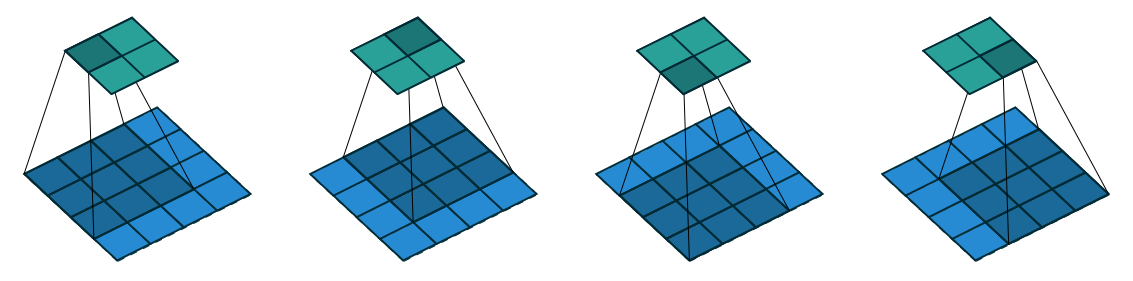
\includegraphics[width=0.9\linewidth]{images/no-padding-unit-stride}
	\caption{Chế độ không đệm, bước nhảy đơn vị}
	\label{fig:no-padding-unit-stride}
\end{figure}

Có 2 loại đệm:
\begin{itemize}
	\item Đệm nửa đảm bảo kích thước ma trận đầu ra bằng kích thước ma trận đầu vào như hình \ref{fig:half-padding-unit-stride1}. Giá trị đệm nửa xác định bằng công thức \ref{eqn:haft-padding}.
	\begin{equation}\label{eqn:haft-padding}
		p = \frac{k-1}{2}
	\end{equation}
	\item Đệm đầy đủ đảm bảo kích thước ma trận đầu ra lớn hơn hoặc bằng kích thước ma trận đầu vào như hình \ref{fig:full-padding-unit-stride}. Giá trị đệm đầy đủ tính bằng công thức \ref{eqn:full-padding}.
	\begin{equation}\label{eqn:full-padding}
		p = k-1
	\end{equation}
\end{itemize}
% TODO: \usepackage{graphicx} required
\begin{figure}
	\centering
	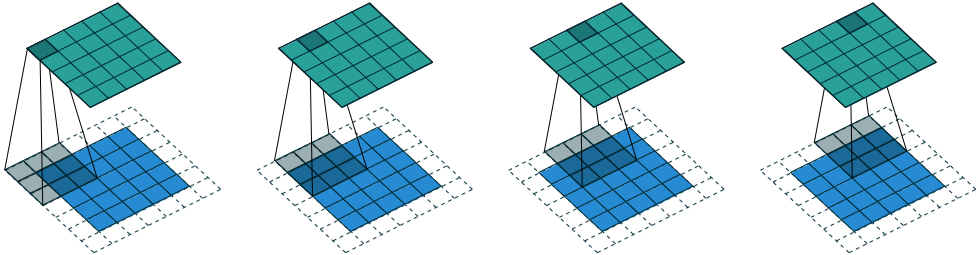
\includegraphics[width=0.9\linewidth]{images/half-padding-unit-stride1}
	\caption{Chế độ đệm nửa, bước nhảy đơn vị}
	\label{fig:half-padding-unit-stride1}
\end{figure}

% TODO: \usepackage{graphicx} required
\begin{figure}
	\centering
	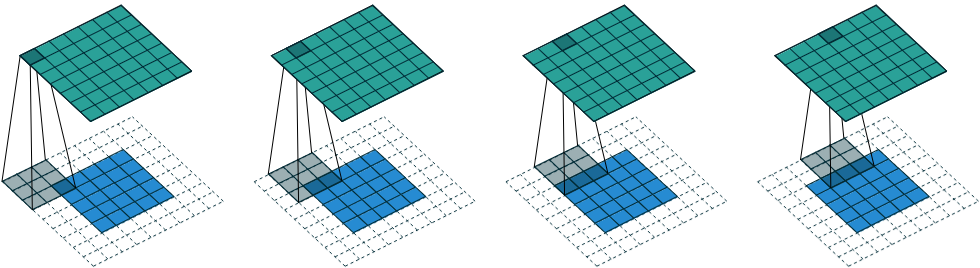
\includegraphics[width=0.9\linewidth]{images/full-padding-unit-stride}
	\caption{Chế độ đệm đầy đủ, bước nhảy đơn vị}
	\label{fig:full-padding-unit-stride}
\end{figure}

\textbf{Thuộc tính bước nhảy}

Bước nhảy là số lượng phần tử giữa hai lần áp dụng tích chập ma trận đầu vào với bộ lọc. Như vậy, thay vì di chuyển 1 điểm ảnh trên ảnh đầu vào trong phép tích chập thông thường, áp dụng bước nhảy sẽ di chuyển ma trận với $s$ điểm ảnh thao tác này được mô tả trong hình \ref{fig:half-padding-stride-2}.

% TODO: \usepackage{graphicx} required
\begin{figure}[h]
	\centering
	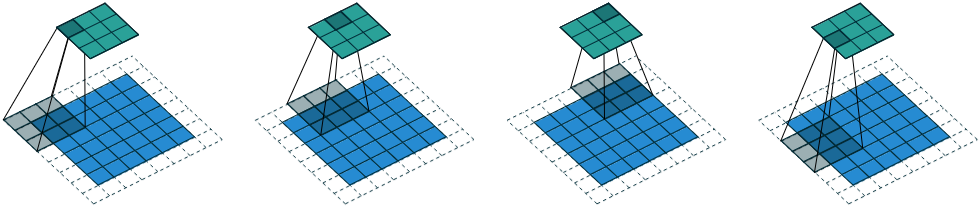
\includegraphics[width=0.9\linewidth]{images/half-padding-stride-2}
	\caption{Chế độ đệm nửa, bước nhảy 2}
	\label{fig:half-padding-stride-2}
\end{figure}

Sử dụng bước nhảy có thể làm giảm kích thước của đầu ra so với đầu vào ban đầu, vì những vị trí không được xem xét. Tuy nhiên, bước nhảy cũng giúp giảm độ phức tạp tính toán và số lượng tham số trong mạng nơ-ron tích chập, đồng thời có thể tạo ra các biểu diễn đặc trưng tổng quát hơn và giảm hiện tượng quá khớp.


Việc kết hợp bước nhảy và đệm tạo ra ma trận với kích thước tính theo công thức \ref{eqn:padding-stride}.

\begin{equation}\label{eqn:padding-stride}
	o = \lfloor{\frac{i-k}{s}}\rfloor + 1
\end{equation}

\textbf{Phép chập khối}

Trong thực tế, việc áp dụng các bộ lọc trên ảnh thường được áp dụng cho cả 3 kênh màu đỏ, lục và lam. Như vậy, bộ lọc hay khối lọc cần có 3 chiều bao gồm màu sắc, chiều cao và chiều rộng. 

Hình \ref{fig:single-filter-block-conv} mô tả ảnh đầu vào kích thước $6 \times 6$ trên hệ màu RGB. Như vậy, đầu vào có thể biểu diễn dạng ma trận kích thước $(6 \times 6 \times 3)$. Khối lọc để áp dụng tương ứng cũng phải có 3 lớp tương ứng với 3 màu đỏ, lục và lam.

% TODO: \usepackage{graphicx} required
\begin{figure}[h]
	\centering
	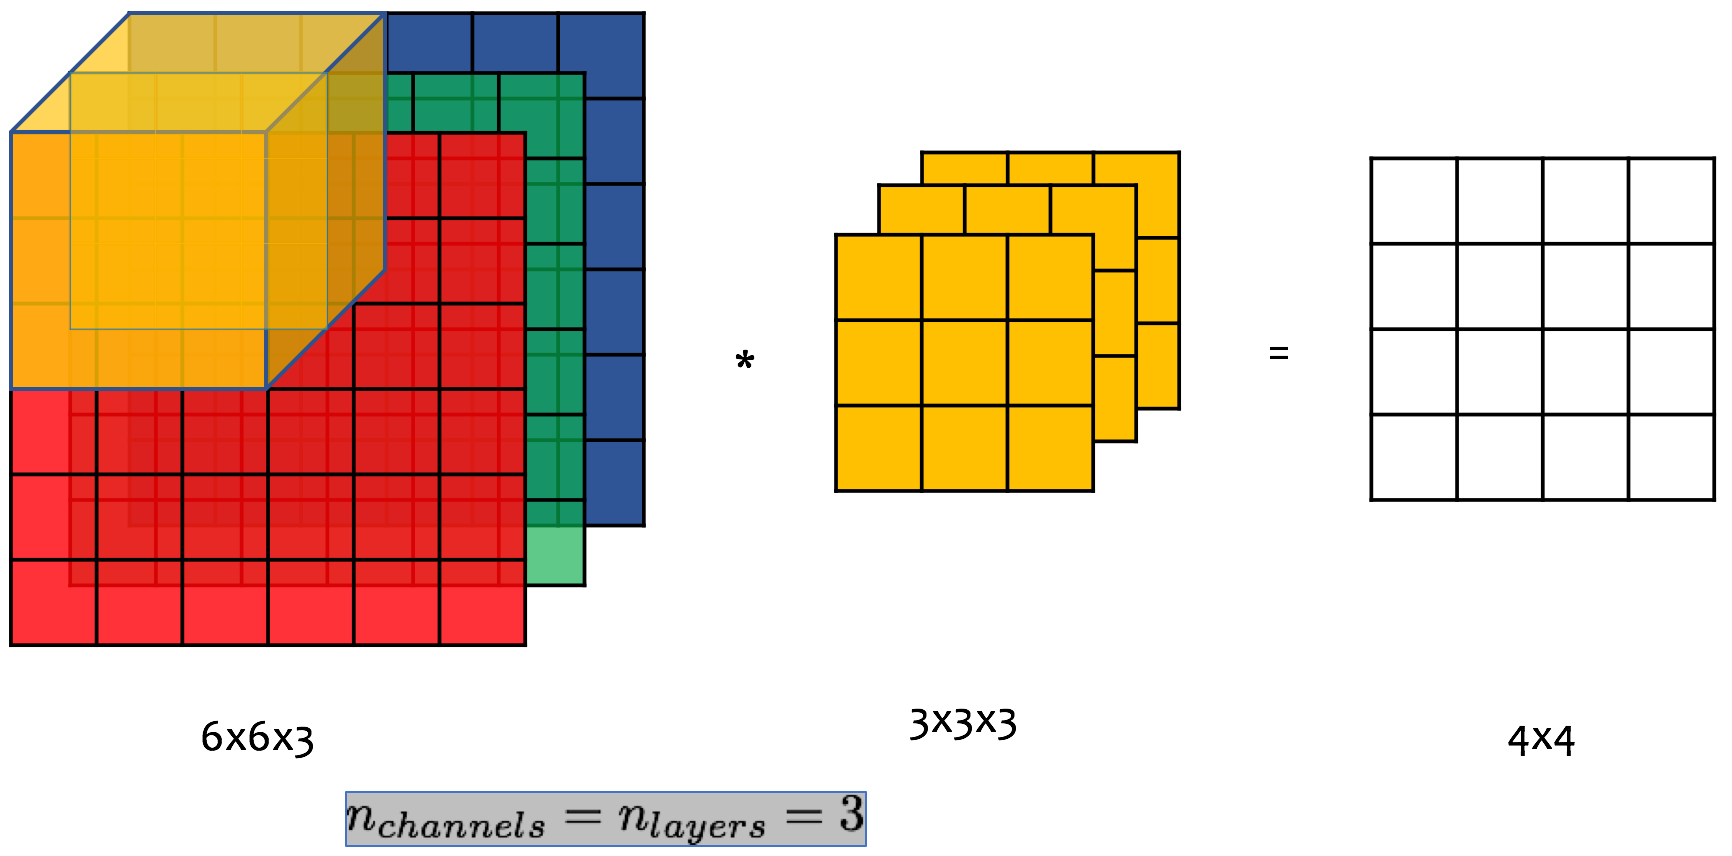
\includegraphics[width=0.8\linewidth]{images/single-filter-block-conv}
	\caption{Phép chập khối \cite{dl_ap_2018}}
	\label{fig:single-filter-block-conv}
\end{figure}

Việc tính toán kết quả sau khi áp dụng khối lọc thực hiện bằng cách dịch chuyển khối lọc trên khối ma trận vào. Mỗi lớp của bộ lọc được chập với diện tích phủ bởi nó trên kênh tương ứng của ma trận vào. Tại một vị trí tương ứng của khối lọc, giá trị tại ô tương ứng của ma trận đầu ra là tổng của các kết quả phép chập trên từng lớp.

Như vậy, dữ liệu đầu vào có thể có nhiều kênh khác nhau, tương ứng với đó, các bộ lọc cũng phải có số kênh tương ứng. Kết quả phép chập giữa ma trận đầu vào $X$ với $n$ kênh và khối lọc $K$ được tính bằng công thức \ref{eqn:block-conv}.

\begin{equation}\label{eqn:block-conv}
	Y = \sum^n_{i=1}X_i\star K_i
\end{equation}

Phép chập có thể được sử dụng để phát hiện và trích xuất đặc trưng trên một hoặc nhiều kênh vào. Ví dụ, để phát hiện đặc trưng trên kênh màu đỏ và bỏ qua kênh màu xanh lục và xanh lam, bộ phát hiện chỉ được đặt ở lớp đầu tiên và giá trị 2 lớp còn lại bằng 0.



\textbf{Phép chập khối với nhiều bộ lọc}

Sau mỗi khối lọc, kết quả thu được sau khi thực hiện chập với ma trận khối đầu vào là một ma trận 2 chiều tương ứng với một đặc trưng của đầu vào. Để thu được nhiều đặc trưng từ ảnh đầu vào hay để sinh ra $d$ đặc trưng khác nhau, có thể sử $d$ khối lọc lần lượt chập với ma trận đầu vào để thu được $d$ ma trận đầu ra, xếp chồng chúng trở thành $d$ kênh đầu ra. Hình \ref{fig:multiple-filter-block-conv} mô tả các thao tác và kết quả sau khi áp dụng khối lọc.

% TODO: \usepackage{graphicx} required
\begin{figure}[h]
	\centering
	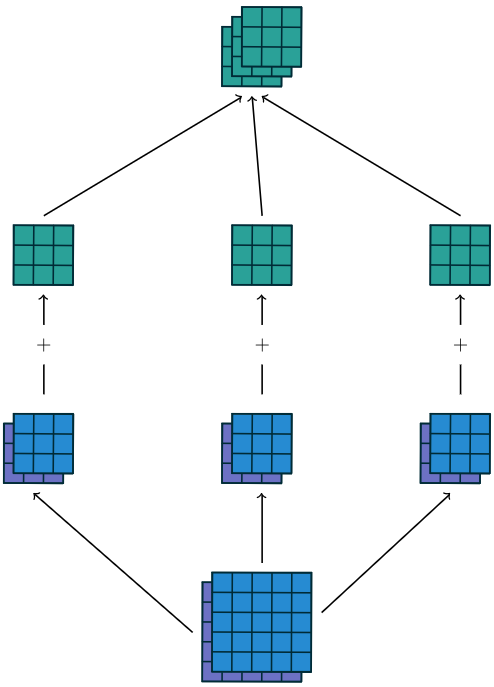
\includegraphics[width=0.6\linewidth]{images/multiple-filter-block-conv}
	\caption{Phép chập nhiều bộ lọc \cite{wei2021}}
	\label{fig:multiple-filter-block-conv}
\end{figure}

Như vậy, thêm vào giá trị hiệu chỉnh $B$ cho từng kênh đầu vào, lớp tích chập có thể được tính tổng quát bằng công thức \ref{eqn:conv-layer}.

\begin{equation}\label{eqn:conv-layer}
	Y_i = B_i + \sum^n_{j=1}X_j \star K_{ij}, i = 1...d 
\end{equation}

\subsubsection{Lớp gộp}
Lớp gộp là một lớp quan trọng giúp giảm kích thước không gian đầu ra của lớp trước đó trong \acrshort{cnn}. 

Mục tiêu chính của lớp gộp là giảm số lượng tham số và tính toán trong mạng nơ-ron, đồng thời giữ lại các đặc trưng quan trọng. Lớp gộp thực hiện điều này bằng cách áp dụng một phép gộp lên các vùng không gian của đầu vào và trích xuất thông tin quan trọng từ những vùng này.

Có hai loại phép gộp phổ biến trong lớp gộp:

\begin{itemize}
	\item Gộp cực đại: phép gộp cực đại lấy giá trị lớn nhất trong mỗi vùng không gian của đầu vào. Nó giúp tìm ra đặc trưng nổi bật nhất trong mỗi vùng và giữ lại thông tin quan trọng. Phép gộp cực đại được mô tả trong hình \ref{fig:max-pooling}.
	\item Gộp trung bình: phép gộp trung bình tính giá trị trung bình của các điểm ảnh trong mỗi vùng không gian của đầu vào. Nó có thể giữ lại thông tin tổng quát về mức độ xuất hiện của đặc trưng trong mỗi vùng phép gộp trung bình được mô tả trong hình \ref{fig:avg-pooling}.
\end{itemize}


% TODO: \usepackage{graphicx} required
\begin{figure}[h]
	\centering
	\begin{subfigure}{.4\textwidth}
		\centering
		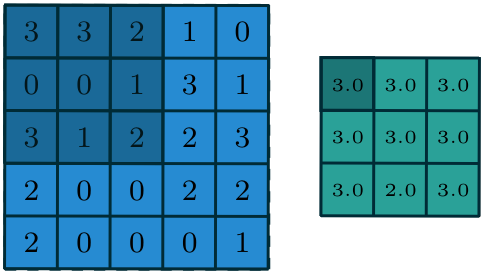
\includegraphics[width=.9\linewidth]{images/max-pooling}
		\caption{Gộp cực đại}
		\label{fig:max-pooling}
	\end{subfigure}

	\begin{subfigure}{.4\textwidth}
		\centering
		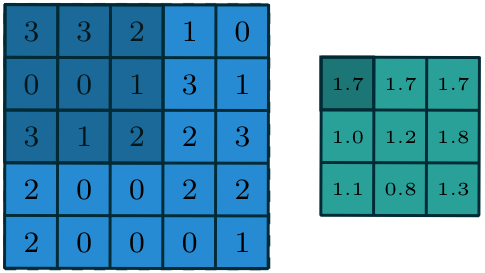
\includegraphics[width=.9\linewidth]{images/avg-pooling}
		\caption{Gộp trung bình}
		\label{fig:avg-pooling}
	\end{subfigure} %
	\caption{Thuật toán gộp cực đại và gộp trung bình với bước nhảy đơn vị}
\end{figure}

Giống như lớp tích chập, lớp gộp cũng có thể sử dụng độ bước nhảy để xác định khoảng cách di chuyển của khung gộp trên ma trận vào. Nếu bước nhảy là 1 hay bước nhảy đơn vị, khung gộp sẽ di chuyển một bước một vị trí trong mỗi lần tính toán. Nếu bước nhảy lớn hơn 1, khung gộp sẽ di chuyển nhanh hơn và kích thước của ma trận kết quả sẽ nhỏ hơn so với đầu vào.

Lớp gộp thường được sử dụng sau mỗi lớp tích chập trong mạng \acrshort{cnn} để giảm kích thước không gian của đặc trưng và tổng quát hóa thông tin. Việc giảm kích thước không gian giúp giảm số lượng tham số và tính toán, đồng thời tạo ra các đặc trưng cấp cao hơn bằng cách tóm tắt thông tin từ các vùng lớn hơn của đầu vào.

Tuy nhiên, lớp gộp cũng có một nhược điểm là gây ra mất mất một số thông tin chi tiết, vì chỉ giữ lại thông tin quan trọng nhất. Điều này có thể làm mất một số thông tin nhỏ nhưng quan trọng, đặc biệt đối với các bài toán yêu cầu độ chính xác cao.

\subsubsection{Lớp kích hoạt}
Lớp kích hoạt trong mạng \acrshort{cnn} là một lớp không có trọng số và thường được đặt sau mỗi lớp tích chập hoặc lớp kết nối đầy đủ trong mạng.

Nguyên lý hoạt động của lớp kích hoạt như sau:

\begin{itemize}
    \item Đầu vào: lớp kích hoạt nhận đầu vào từ lớp trước đó trong mạng nơ-ron. Đầu vào có thể là một tensor hoặc một ma trận, tùy thuộc vào kiến trúc của mạng nơ-ron.
    \item Hàm kích hoạt: lớp kích hoạt áp dụng một hàm kích hoạt phi tuyến tính lên đầu vào. Hàm kích hoạt này thường được chọn để giới hạn đầu ra và tạo độ không tuyến tính cho mạng nơ-ron. Một số hàm kích hoạt phổ biến bao gồm:
    \begin{itemize}
        \item Hàm ReLU (Rectified Linear Unit): $f(x) = max(0, x)$. Nó giữ nguyên giá trị không âm và bỏ qua các giá trị âm.
        \item Hàm Sigmoid: $f(x) = \frac{1}{1 + e^{-x}}$. Nó chuyển đổi giá trị đầu vào thành một phạm vi từ $0$ đến $1$, thường được sử dụng trong các bài toán phân loại nhị phân.
        \item Hàm Tanh: $f(x) = \frac{e^x - e^{-x}}{e^x +x e^{-x}}$. Tương tự như hàm sigmoid, nhưng đầu ra nằm trong khoảng từ $-1$ đến $1$.
        \item Hàm Softmax: $f(x_i) = \frac{e^{x_i}}{\sum^n_j e^{x_j}}$, với $i$ là chỉ số của đầu ra và $j$ là chỉ số của tất cả các đầu ra. Hàm softmax thường được sử dụng trong bài toán phân loại đa lớp để chuyển đổi đầu vào thành các xác suất phân loại.
    
    \end{itemize}
    \item Đầu ra: kết quả của lớp kích hoạt là đầu ra của lớp này, được truyền tới lớp tiếp theo của mạng.
\end{itemize}
    
Lớp kích hoạt chủ yếu được sử dụng để tạo độ không tuyến tính trong mạng nơ-ron và giúp mô hình học được các đặc trưng phức tạp và biểu diễn các mô hình quan hệ phi tuyến. Nó cũng giúp giới hạn đầu ra trong một phạm vi nhất định và tạo ra các đầu ra dễ hiểu và dễ xử lý cho các lớp tiếp theo.

Các hàm kích hoạt và vị trí của lớp kích hoạt trong mạng nơ-ron có thể được điều chỉnh tùy thuộc vào bài toán cụ thể và kiến trúc mạng nơ-ron.

\subsubsection{Lớp kết nối đầy đủ}
Lớp kết nối đầy đủ còn được gọi là lớp đầu ra trong mạng nơ-ron, là một trong những loại lớp quan trọng trong kiến trúc mạng nơ-ron truyền thẳng.

Lớp kết nối đầy đủ thường được sử dụng trong các mạng nơ-ron truyền thẳng để tạo ra đầu ra cuối cùng của mạng. Nó giúp mô hình học được các mối quan hệ phức tạp giữa đầu vào và đầu ra. Các lớp kết nối đầy đủ thường được sử dụng trong các bài toán như phân loại ảnh, nhận dạng giọng nói, bài toán dự báo, và nhiều bài toán khác.

Có thể nói, sự khác biệt duy nhất giữa lớp kết nối đầy đủ và lớp tích chập là các nơ-ron trong lớp tích chập chỉ được kết nối tới một phần của đầu vào tuy vậy, cả lớp kết nối đầy đủ và lớp tích chập đều được tính toán như nhau. Vì vậy, ta có thể thay thế lớp kết nối đầy đủ bằng lớp tích chập có kích thước bằng kích thước đầu vào.

Một số kiến trúc mạng nơ-ron sử dụng nhiều lớp kết nối đầy đủ liên tiếp nhau để tạo thành một mạng nơ-ron sâu. Trong các mạng nơ-ron sâu, thông qua việc kết hợp nhiều lớp kết nối đầy đủ với các hàm kích hoạt phi tuyến tính, mô hình có khả năng học được các đặc trưng phức tạp và biểu diễn các mô hình quan hệ phi tuyến giữa đầu vào và đầu ra.

\subsection{Hoạt động của mạng nơ-ron tích chập}
\subsubsection{Hàm mất mát}

Hàm mất mát là một hàm số được sử dụng trong quá trình huấn luyện mô hình máy học để đo lường sự khác biệt giữa các dự đoán của mô hình và giá trị thực tế của dữ liệu đích. Mục tiêu của việc tối ưu hàm mất mát là điều chỉnh các tham số của mô hình để giảm thiểu sai số giữa dự đoán và giá trị thực tế.

Hàm mất mát thường được xây dựng dựa trên mục tiêu cụ thể của vấn đề máy học mà bạn đang giải quyết.

Trong bài toán phát hiện đối tượng, hai hàm mất mát quan trọng nhất là hàm mất mát về lớp đối tượng và hàm mất mát về hộp bao.

Gọi vùng hình ảnh chiếm chỗ thực tế của đối tượng là $A$, vùng hình ảnh dự đoán được của mô hình là $A'$, có thể dễ dàng tính toán được vùng giao và hợp của hai vùng $A$ và $A'$. Hàm mất mát về hộp bao có thể được tính toán từ hai vùng này theo công thức \ref{eqn:iou}.

\begin{equation} 
	\label{eqn:iou}
	IoU=\frac{A\cup A'}{A\cap A'}
\end{equation}

Mọi thay đổi liên quan đến vị trí hoặc hình dạng hộp bao đều làm giảm $IoU$, vì vậy, $IoU$ có thể được sử dụng đánh giá độ chính xác về cả vị trí và hình dạng hộp bao, tối ưu các tham số nhằm sinh $IoU$ cao hơn giúp tăng độ chính xác của mô hình khi xác định hộp bao của vật thể.

Đối với hàm mất mát về lớp đối tượng, hàm mất mát có thể thuộc dạng $1 - 0$, nghĩa là đúng hoặc sai trong dự đoán, hoặc sử dụng phương pháp đo lường sự khác biệt giữa phân phối xác suất dự đoán của mô hình với phân phối xác suất thực tế của các lớp.

Gọi $y_i$ là xác suất của lớp thứ $i$ trong tập dữ liệu, $y'_i$ là xác suất của lớp $i$ trong tập dự đoán, có thể xây dựng hàm mất mát như công thức \ref{eqn:ce-loss}. Như vậy, nếu xác suất dự đoán chính xác càng thấp, giá trị mất mát càng nhỏ và ngược lại.

\begin{equation}
	\label{eqn:ce-loss}
	L_{CE} = - \sum_{i = 1}^{n}y_ilog(y'_i)
\end{equation}

\subsubsection{Quá trình lan truyền thuận}

Quá trình lan truyền thuận là quá trình dữ liệu được đưa vào qua lớp đầu vào. Các trọng số và hệ số điều chỉnh của mạng được sử dụng để tính toán giá trị đầu ra của mỗi nơ-ron trong lớp tiếp theo.

Trong \acrshort{cnn} với nhiều lớp tích chập, đầu ra của các lớp tích chập được đưa vào hàm kích hoạt phi tuyến tính trước khi làm đầu vào cho các lớp tiếp theo. Như vậy, kết quả của lớp tích chập \ref{eqn:conv-layer} sẽ được đưa vào hàm kích hoạt trước khi làm đầu vào cho các tầng tiếp theo. 

Đầu ra của lớp tích chập cuối cùng có thể được xử lý để đưa ra kết quả của mạng với đầu vào tương ứng hoặc được đưa vào các mạng tiếp theo để phục vụ mục đích bài toán như phân loại, ...



\subsubsection{Quá trình lan truyền nghịch}
Trong quá trình huấn luyện mạng, từ kết quả của quá trình lan truyền thuận, có thể xác định được sự chênh lệch về kết quả đoán nhận được so với kết quả thực tế. Quá trình lan truyền nghịch được sử dụng để tinh chỉnh giá trị trọng số trong các nhân lớp tích chập và hệ số tinh chỉnh tương ứng. 

Độ lệch trong số $\omega_{ab}$ có thể tính theo công thức \ref{eqn:back-prop1}.

\begin{equation}\label{eqn:back-prop1}
	\frac{dE}{dw_{ab}} = \sum^{N-m}_{i=0}\sum^{N-m}_{j=0} \frac{dE}{dx^l_{ij}} \frac{dx^l_{ij}}{d\omega_{ab}} =  \sum^{N-m}_{i=0}\sum^{N-m}_{j=0} \frac{dE}{dx^l_{ij}} y^{l-1}_{(i+a)(j+b)}
\end{equation}

Độ dốc $\frac{dE}{dx^l_{ij}}$ được tính bằng công thức \ref{eqn:back-prop2}:
\begin{equation}\label{eqn:back-prop2}
	\frac{dE}{dx^l_{ij}} = \frac{dE}{dy^l_{ij}}\frac{dy^l_{ij}}{dx^l_{ij}} =  \frac{dE}{dy^l_{ij}} \frac{d}{dx^l_{ij}}(\sigma (x^l_{ij})) = \frac{dE}{dy^l_{ij}}\sigma' ((x^l_{ij}))
\end{equation}

Ngoài các giá trị trọng số phải tính hiện tại, quá trình huấn luyện còn cần biết độ thay đổi của tham số đầu vào lớp hiện tại để tiếp tục áp dụng cho các lớp trước đó. Độ thay đổi được tính bằng công thức \ref{eqn:back-prop3}.

\begin{equation}\label{eqn:back-prop3}
	\frac{dE}{dy^{l-1}_{ij}} = \sum^{m-1}_{a=0} \sum^{m-1}_{b=0} \frac{dE}{dx^l_{(i-a)(j-b)}} \frac{dx^l_{(i-a)(j-b)}}{dy^{l-1}_{ij}} = \sum^{m-1}_{a=0} \sum^{m-1}_{b=0} \frac{dE}{dx^l_{(i-a)(j-b)}}\omega_{ab}
\end{equation}

\subsection{Các độ đo}
Các dự đoán sinh ra từ \acrshort{cnn} có thể thuộc nhiều kết quả khác nhau nhưng bằng việc sinh ra kết quả nhị phân (đúng/sai) cho tất cả kết quả có thể, việc phân tích kết quả sẽ trở nên đơn giản hơn với các kết quả $TP$, $TN$, $FP$, $FN$:

\begin{itemize}
	\item True Positive ($TP$): số lượng mẫu mà mô hình dự đoán "đúng" là "đúng".
	\item False Negative ($FN$): số lượng mẫu mà mô hình dự đoán "sai" là "đúng".
	\item False Positive ($FP$): số lượng mẫu mà mô hình dự đoán "đúng" là "sai".
	\item True Negative ($TN$): số lượng mẫu mà mô hình dự đoán "sai" là "sai".
\end{itemize}

Dựa trên các kết quả trên, một số thông số quan trọng được sử dụng để đánh giá hiệu suất của mô hình qua các độ đo.

Ma trận nhầm lẫn (Confusion matrix) là một công cụ thường được sử dụng để đánh giá hiệu của mô hình phân loại. Ma trận hiển thị tần suất của các dự đoán của mô hình so với thực tế trong tập kiểm tra, giúp nhận biết số lượng và tỉ lệ đúng hay sai của các dự đoán bởi mô hình. Cấu trúc của một ma trận nhầm lẫn được mô tả trong hình \ref{fig:confusion-matrix}.

\begin{figure}
	\centering
	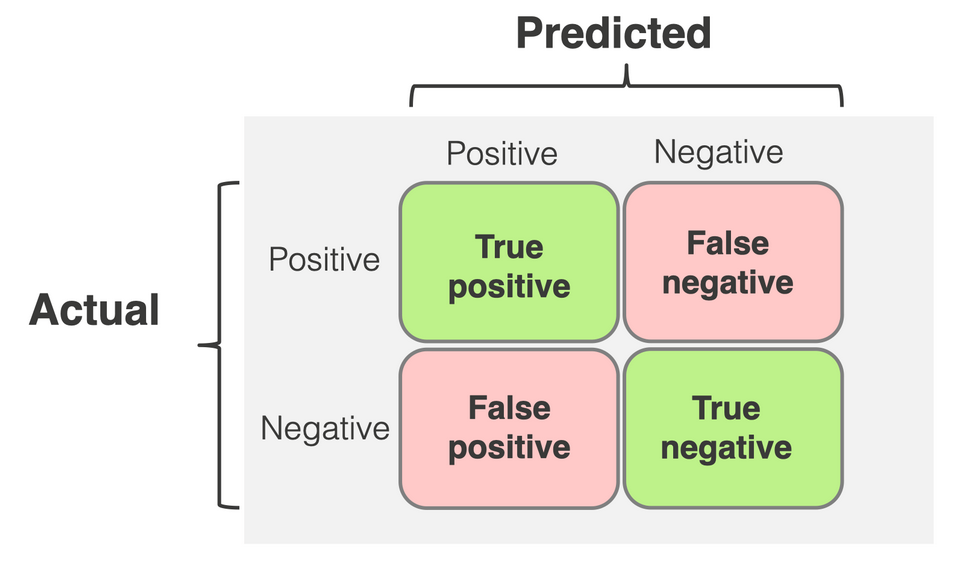
\includegraphics[width=0.7\linewidth]{images/confusion-matrix}
	\caption{Ma trận nhầm lẫn}
	\label{fig:confusion-matrix}
\end{figure}


Độ chính xác $Accuracy$ là tỷ lệ phần trăm của số lượng dự đoán chính xác trên tổng số lượng dự đoán. Độ chính xác được tính bằng công thức \ref{eqn:acc}.
\begin{equation}
	\label{eqn:acc}
	Accuracy = \frac{TP + TN}{TP + TN + FP + FN}
\end{equation}

Độ chính xác dương tính $Precision$ đo lường tỷ lệ giữa số lượng dự đoán dương tính chính xác và tổng số lượng dự đoán dương tính. Đây là tỉ lệ giữa số lượng dự đoán "đúng" chính xác và tổng số lượng dự đoán theo công thức \ref{eqn:prec}.

\begin{equation}
	\label{eqn:prec}
	Precision = \frac{TP}{TP + FP}
\end{equation}	

Độ nhớ tìm kiếm $Recall$ còn được gọi là độ nhạy, đo lường tỷ lệ giữa số lượng dự đoán dương tính chính xác và tổng số lượng thực tế dương tính. Đây là tỉ lệ giữa số lượng dự đoán "đúng" chính xác và tổng số lượng dự đoán đúng thực tế.
\begin{equation}
	\label{eqn:recall}
	Recall = \frac{TP}{TP + FN}
\end{equation}	
	
Điểm $F\mathit{1}$ là một đánh giá tổng hợp, kết hợp giữa Độ chính xác dương tính và độ nhạy. Nó đo lường sự cân bằng giữa độ chính xác dương tính và độ nhạy. 
\begin{equation}
	\label{eqn:f1}
	F\mathit{1}_{score} = \frac{2 * (Precision * Recall)}{(Precision + Recall)}
\end{equation}

\subsection{Hiện tượng quá khớp}

Xét một mạng nơ-ron bất kỳ, khi mạng càng sâu hay số lớp trong mạng càng tăng lên, thì nó càng có khả năng khớp với dữ liệu phức tạp cao như hình \ref{fig:overfitting}. Hiện tượng quá khớp xảy ra khi mạng CNN có số lớp quá sâu so với dữ liệu đơn giản.

Theo \cite{karpathy}, có nhiều cách giảm thiểu hiện tượng quá khớp tốt hơn việc giảm độ sâu của mạng. Tuy nhiên, đối với hệ thống phần cứng giới hạn, giảm độ sâu của mạng đến mức tối thiểu mà vẫn đảm bảo khả năng suy đoán sẽ mang lại thời gian tính toán nhanh hơn.

\begin{figure}[h]
	\centering
	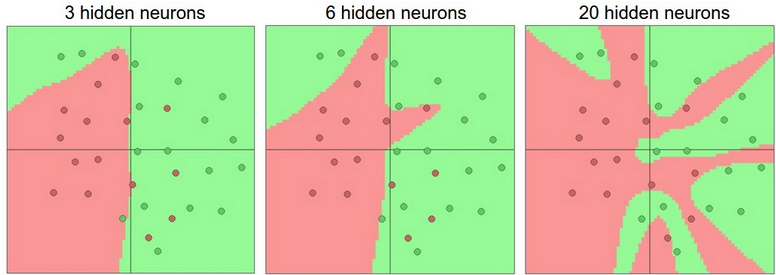
\includegraphics[width=0.7\linewidth]{images/overfitting}
	\caption{Quá khớp trong mạng nơ-ron}
	\label{fig:overfitting}
\end{figure}

\section{Mô hình \acrshort{yolo}}

\acrshort{yolo} là một mô hình phổ biến trong lĩnh vực nhận diện đối tượng và phát hiện vị trí đối tượng trong ảnh và băng hình. Mô hình \acrshort{yolo} có khả năng phân loại và định vị các đối tượng trong một khung hình duy nhất một cách nhanh chóng và chính xác.

Ý tưởng chính trong mô hình \acrshort{yolo} bao gồm:
\begin{itemize}
	\item Sử dụng phương pháp phát hiện một bước, tức từ ảnh đầu vào thực hiện phát hiện vật thể và hộp bao trong một mạng duy nhất.
	\item Ảnh đầu vào được chia thành các ô với kích thước cố định. Mỗi ô vuông trong lưới sẽ dự đoán hộp bao và lớp vật thể mà tâm của nó nằm trong ô đó.
	\item Mỗi hộp bao được dự đoán bằng 4 tham số: tọa độ tâm, chiều rộng và chiều cao cùng một giá trị độ tin cậy thể hiện chắc chắn trong đó chứa vật thể.
	Mội hộp bao cũng kèm theo một véc-tơ chứa xác suất của các loại vật thể nằm trong ô đó.
	
	\item Hàm mất mát bao gồm nhiều thành phần:
	\begin{itemize}
		\item Mất mát định vị: đo lường sự khác biệt giữa dự đoán và thực tế vị trí của hộp bao.
		\item Mật mát độ tin cậy: đo lường sự khác biệt giữa độ tin cậy của hộp bao dự đoán so với thực tế.
		\item Mất mát dự đoán lớp: đo lường sự khác biệt giữa véc tơ xác suất lớp trong dự đoán và thực tế.
	\end{itemize}
	\item \acrshort{yolo} sử dụng \acrshort{cnn} sâu để trích xuất đặc trưng từ ảnh đầu vào.
	\item Loại bỏ các hộp bao trùng lặp sử dụng kỹ thuật NMS giúp lấy ra hộp bao tin cậy nhất cho dự đoán.
	\item Hỗ trợ nhiều kích thước vật thể bằng cách sử dụng nhiều biểu đồ đặc trưng ở độ phân giải khác nhau.
\end{itemize}

\subsection{Kiến trúc mạng của mô hình}

Việc phát hiện vật thể trở nên rất thách thức đối với các vật thể nhỏ. Một phương pháp dễ hiểu là sinh đặc trưng với từng tỉ lệ khác nhau như kim tự tháp trên mạng. Tuy nhiên, phương pháp này gây lãng phí tài nguyên tính toán và bộ nhớ. Vì vậy, mạng đặc trưng kim tự tháp ra đời với mục tiêu cân bằng giữa độ chính xác và tốc độ xử lý.

Mạng đặc trưng kim tự tháp bao gồm một đường từ dưới lên và một luồng từ trên xuống. Đường từ dưới lên thực hiện trích xuất đặc trưng. Càng lên cao độ phân giải càng giảm và giá trị thông tin về ngữ cảnh càng cao. Luồng tiếp theo từ trên xuống có chức năng xây dựng các lớp có độ phân giải cao từ các lớp có thông tin ngữ cảnh cao như trong hình \ref{fig:fpn}. Các mô hình sử dụng \acrshort{cnn} như \acrshort{yolo} sử dụng chính xác kỹ thuật này với các cải tiến để lấy ra đặc trưng từ ảnh đầu vào một cách chi tiết và tổng quát nhất cho các kích thước ảnh khác nhau.

% TODO: \usepackage{graphicx} required
\begin{figure}[h]
	\centering
	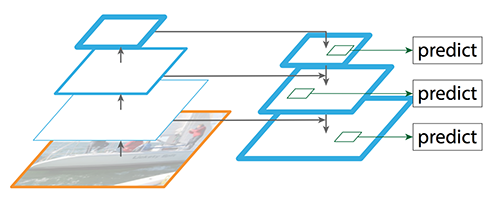
\includegraphics[width=0.8\linewidth]{images/fpn}
	\caption{Mô hình đặc trưng kim tự tháp}
	\label{fig:fpn}
\end{figure}

Kiến trúc mạng \acrshort{yolo} đã trải qua nhiều phiên bản và cải tiến, bao gồm \acrshort{yolo}v1, \acrshort{yolo}v2, \acrshort{yolo}v3 đến \acrshort{yolo}v8. Các phiên bản hiện nay của \acrshort{yolo} được mô tả trong hình \ref{fig:yolov8-structure} bao gồm 3 lớp chính: Lớp xương sống, lớp cổ và lớp đầu trong đó, lớp xương sống và lớp cổ được triển khai theo kiến trúc dạng kim tự tháp để trích xuất đặc trưng.

\begin{figure}[h]
	\centering
	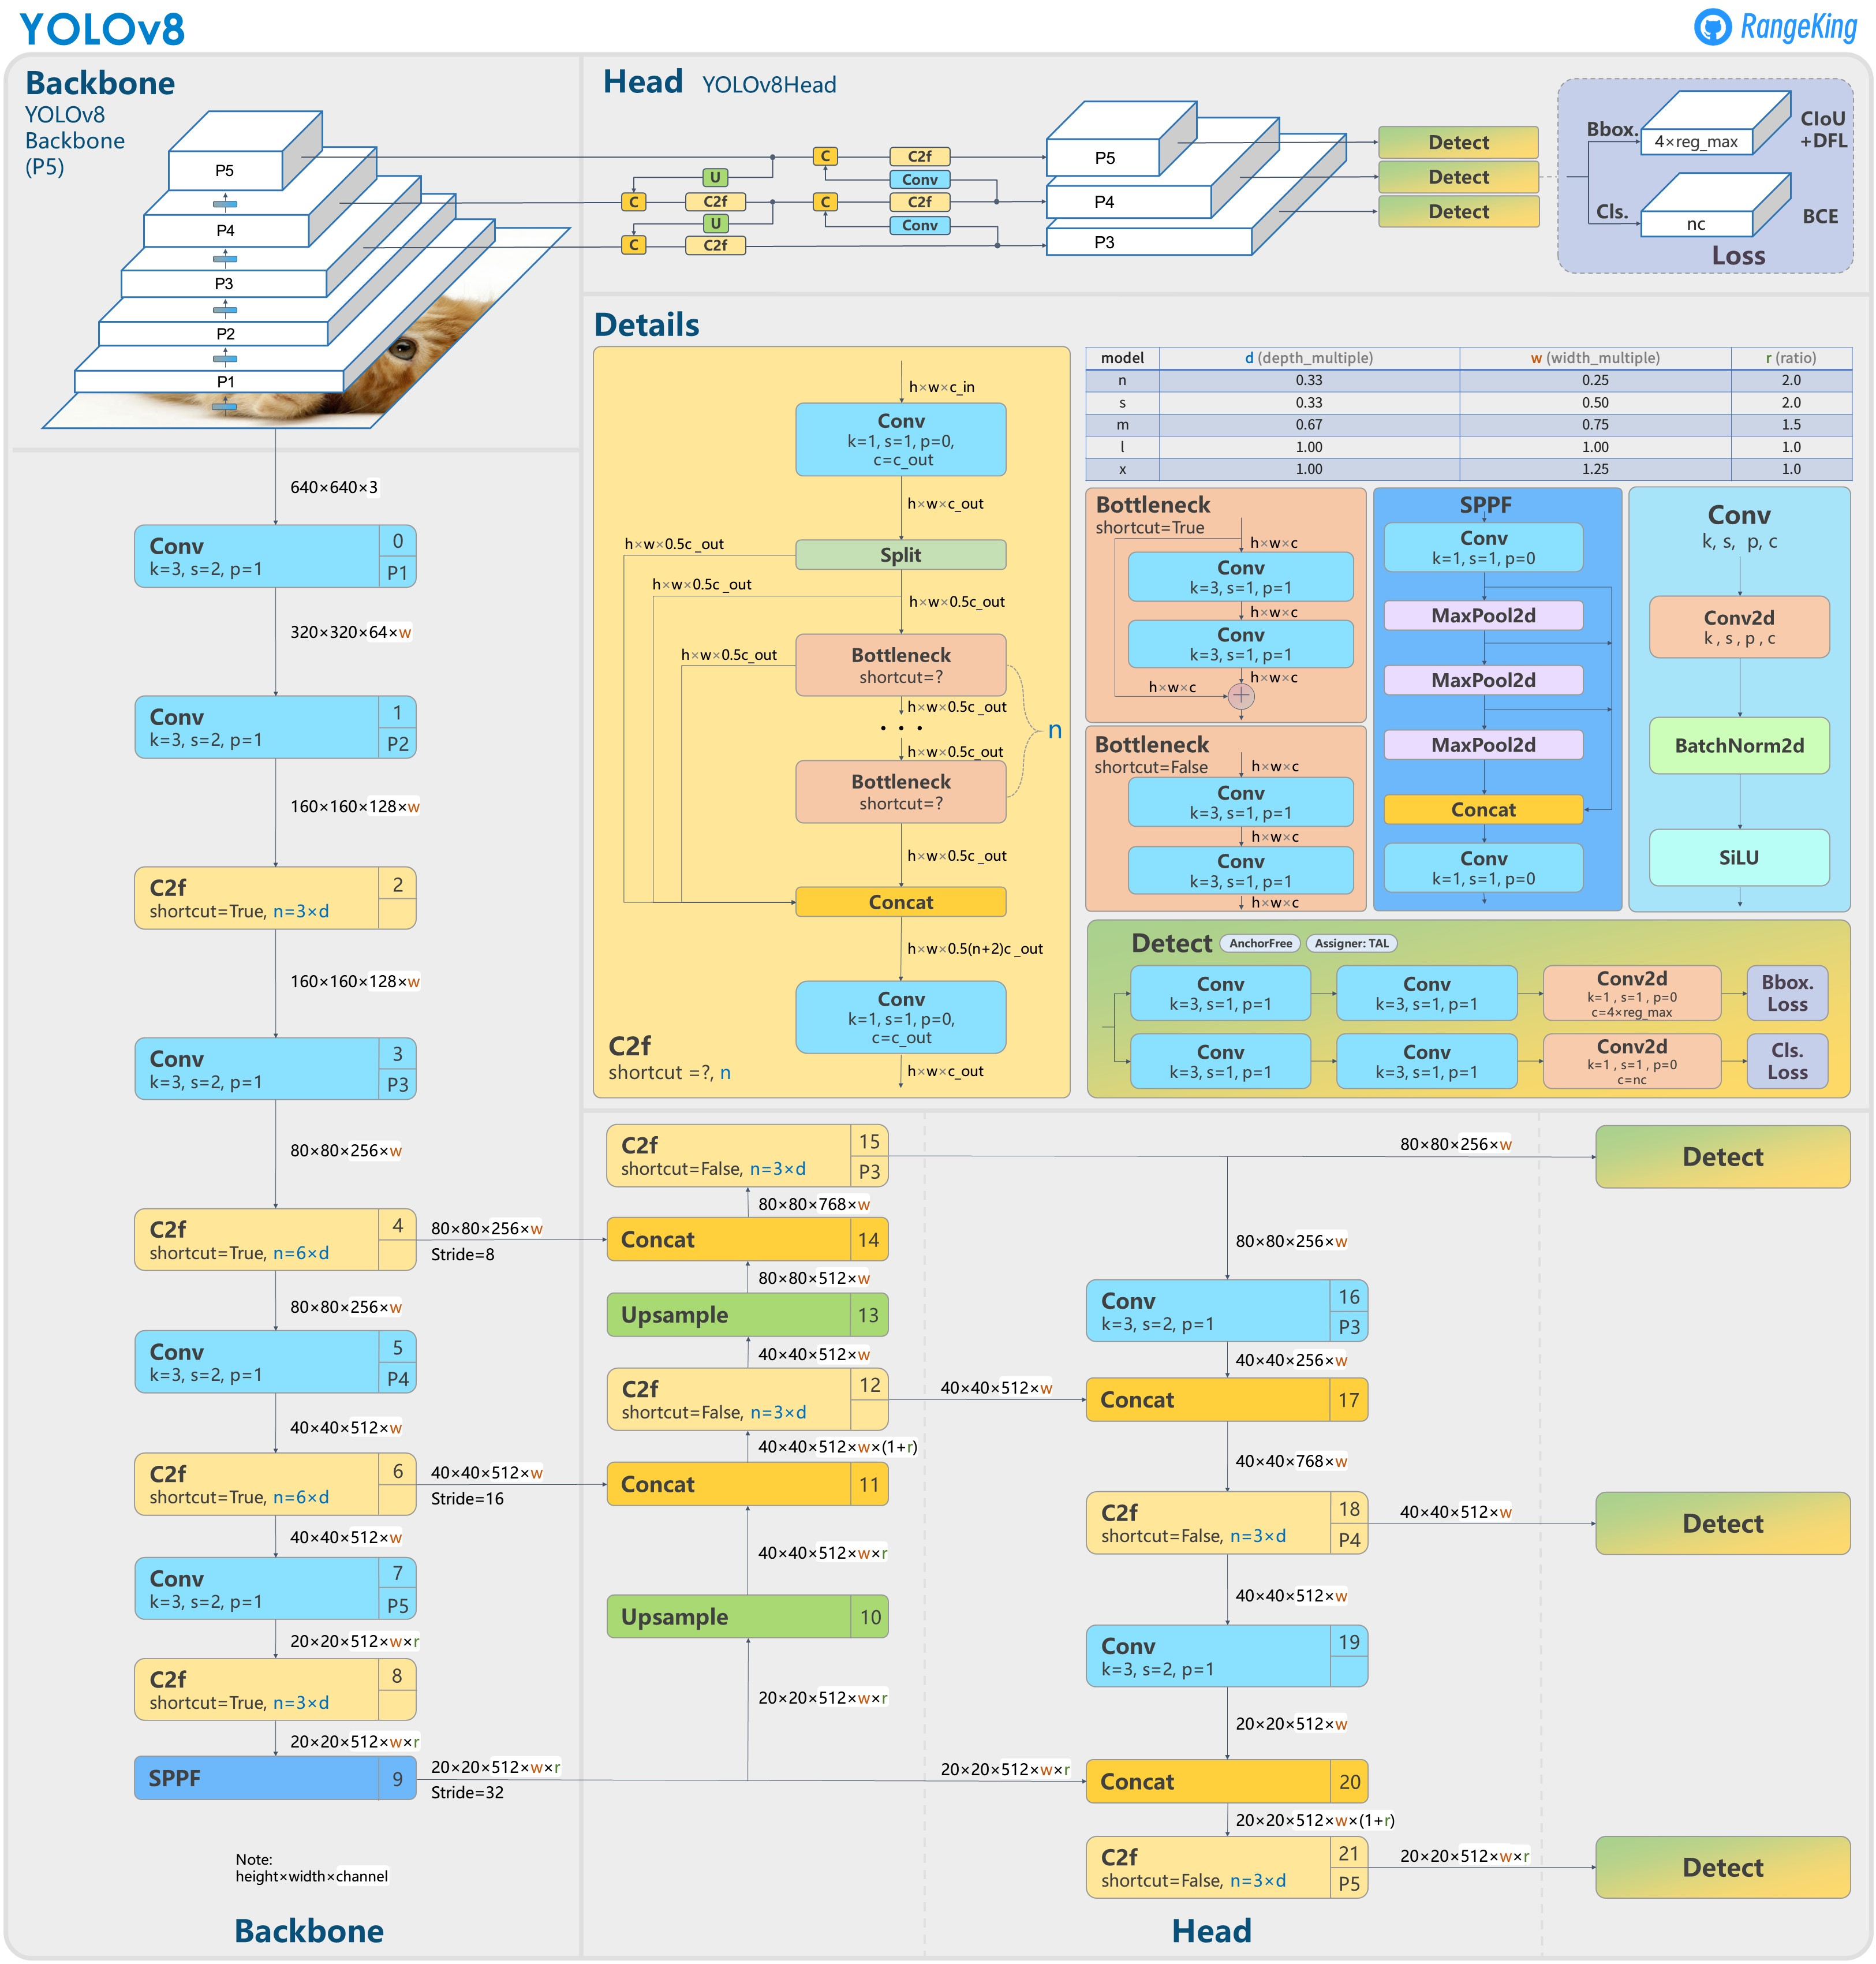
\includegraphics[width=1\linewidth]{images/yolov8-network.png}
	\caption{Cấu trúc mạng \acrshort{yolo}v8 và cấu hình kích thước}
	\label{fig:yolov8-structure}
\end{figure}

\subsubsection{Lớp xương sống}

Lớp xương sống (Backbone) trong \acrshort{yolo}v8 có nhiệm vụ trích xuất các đặc trưng từ hình ảnh đầu vào. Nó bao gồm nhiều lớp tích chập và các mô đun khác để giảm kích thước không gian của hình ảnh trong khi tăng chiều sâu của các đặc trưng.

Lớp lớp tích chập Conv sử dụng nhân $3\times3$, sải bước $s=2$ và đệm $p = 1$ giúp giảm kích thước không gian đi 4 lần.

Lớp C2f là mô đun tích chập được nối tắt, giúp tối ưu tính toán và duy trì các đặc trưng ban đầu.

Lớp SPPF là mô đun gộp giúp giảm kích thước không gian.

\subsubsection{Lớp cổ}

Lớp cổ (Neck) trong \acrshort{yolo}v8 là lớp trung gian giúp kết hợp các đặc trưng từ lớp xương sống. Các quá trình từ trên xuống và từ dưới lên giúp kết hợp thông tin từ các cấp độ khác nhau của lớp xương sống, giúp lấy được cả thông tin không sâu sắc ở độ phân giải cao và các thông tin sâu sắc với độ phân giải thấp.

Lớp Upsample nhận ma trận đầu vào và tăng kích thước của nó lên 4 lần, giúp kết hợp với ma trận đầu vào kích thước cao hơn trong lớp xương sống qua lớp kết nối Concat.

\subsubsection{Lớp đầu}

Lớp đầu (Detection Head) trong \acrshort{yolo}v8 là lớp chịu trách nhiệm cuối cùng trong việc phát hiện ra các vật thể. Nó bao gồm các lớp tích chập để dự đoán hộp bao và các lớp tương ứng.

\subsection{Hàm mất mát}

Với hàm mất mát, mô hình \acrshort{yolo} sử dụng một hàm mất mát kết hợp giữa các thành phần như mất mát định vị, mất mát phân tán và mất mát lớp. Hàm mất mát này giúp tối ưu hóa mô hình và cải thiện độ chính xác của các dự đoán.

Với hàm mất mát định vị, \acrshort{yolo}v8 sử dụng chỉ số đo lường mức độ chồng chéo giữa hộp bao dự đoán và hộp bao thực tế bằng công thức \ref{eqn:iou}.

Trong hàm mất mát để đánh giá xác suất lớp, \acrshort{yolo}v8 sử dụng BCE theo công thức \ref{eqn:bce-loss}.

\begin{equation}
	\label{eqn:bce-loss}
	BCE(p,y)=−[y⋅log(p)+(1−y)⋅log(1−p)]
\end{equation}

Trong đó, $p$ lá xác suất dự đoán và $y$ là nhãn thật (0 hoặc 1).

Việc tập trung vào các hộp bao khó dự đoán phụ thuộc rất nhiều vào hàm mất mát phân tán DFL. DFL giúp tối ưu hóa độ chính xác của dự đoán trong các hộp bao sử dụng công thức \ref{eqn:dfl-loss}.

\begin{equation}
	\label{eqn:dfl-loss}
	DFL(p_t)=-\alpha_t*(1-p_t)^\gamma * log(p_t)
\end{equation}

\begin{itemize}
	\item $p_t$ là xác suất dự đoán đúng:
		$$
		p_t =
		\left\{ 
		\begin{array}{l}
			p\ \ \ \ \ \ \ \ \ \ \text{nếu}\ y = 1 \\
			1-p\ \ \ \text{nếu}\ y = 0
		\end{array} 
		\right.
		$$
	\item $a_t$ là hệ số trọng số để cân bằng các lớp:
		$$
		a_t =
		\left\{ 
		\begin{array}{l}
			a\ \ \ \ \ \ \ \ \ \ \text{nếu}\ y = 1 \\
			1-a\ \ \ \text{nếu}\ y = 0
		\end{array} 
		\right.
		$$	
	\item $\gamma$ là tham số điều chỉnh mức độ tập trung vào các dự đoán khó.		
\end{itemize}

\subsection{Đánh giá hiệu suất của mô hình}

Qua các phiên bản, mô hình \acrshort{yolo} ngày càng được cải thiện. Hình \ref{fig:yolov8-better} cho thấy các phiên bản \acrshort{yolo} ngày càng được cải thiện với lượng tham số nhỏ hơn nhanh hơn nhưng hiệu suất lại cao hơn.


\begin{figure}[h]
    \centering
    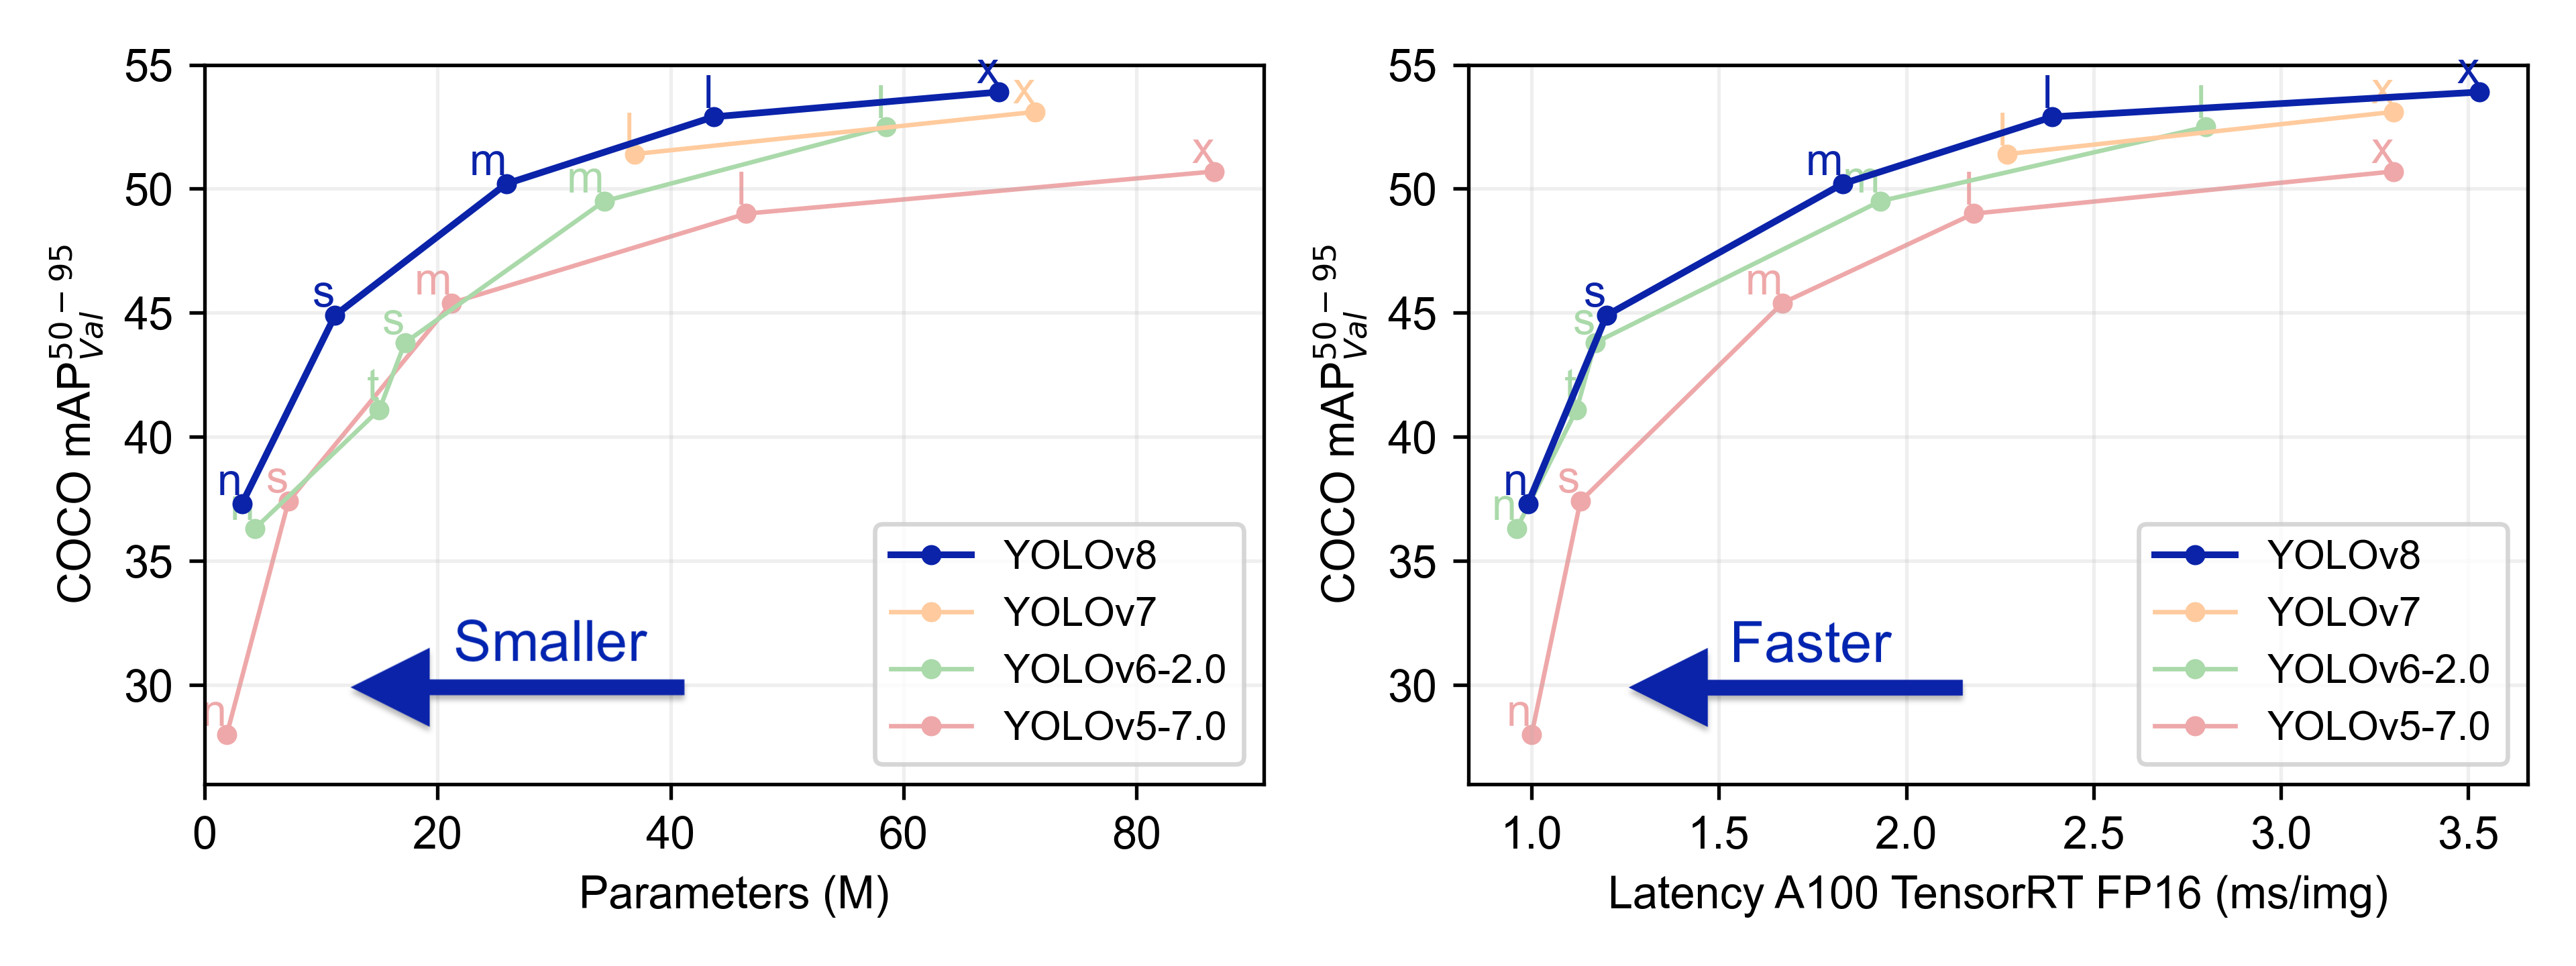
\includegraphics[width=0.75\linewidth]{images/yolov8-better.png}
    \caption{Hiệu suất của mô hình \acrshort{yolo} so với các phiên bản trước đó}
    \label{fig:yolov8-better}
\end{figure}


\subsection{Các tham số cấu hình mạng \acrshort{yolo}}

Đối với mô hình \acrshort{yolo}v8, mô hình có thể được điều chỉnh với các kích thước khác nhau với các tham số trong hình \ref{fig:yolov8-structure}.

Với kích thước lớn - L, mô hình có khả năng học sâu hơn và đưa ra kết quả chính xác hơn. Tuy nhiên, dữ liệu đầu vào cần đa dạng và số lượng lớn hơn để có thể lấy ra những đặc trưng một cách chung nhất. Đối với số lượng mẫu nhỏ, để tránh tình trạng quá khớp, kích thước nhỏ như s, n sẽ phù hợp hơn.

\subsection{So sánh \acrshort{yolo} và \acrshort{cnn} trong phát hiện vật thể}


\subsubsection{Kiến trúc mạng}
\acrshort{cnn} là một kiến trúc mạng nơ-ron sử dụng các tầng tích chập và tầng kết nối đầy đủ để học các đặc trưng của ảnh. \acrshort{cnn} thường sử dụng một số tầng tích chập để trích xuất đặc trưng và sau đó sử dụng các tầng kết nối đầy đủ để phân loại ảnh.

\acrshort{yolo} là một kiến trúc \acrshort{cnn} được thiết kế đặc biệt cho việc phát hiện và định vị đối tượng trong ảnh. \acrshort{yolo} chia ảnh thành các lưới, dự đoán các hộp giới hạn và lớp đối tượng cho mỗi lưới. Các lớp tích chập trong mạng được sử dụng để trích xuất đặc trưng và dự đoán đồng thời các hộp giới hạn và lớp đối tượng.

\subsubsection{Tốc độ}

Với \acrshort{cnn}, việc phân loại và nhận dạng đối tượng được thực hiện trong các lớp cuối cùng của mạng. Điều này có nghĩa là \acrshort{cnn} phải đi qua toàn bộ hình ảnh để đưa ra dự đoán, do đó, tốc độ của \acrshort{cnn} thường chậm hơn so với \acrshort{yolo}.

\acrshort{yolo} sử dụng một phương pháp phát hiện một bước để dự đoán đồng thời các hộp giới hạn và lớp đối tượng trên toàn bộ ảnh. Điều này giúp \acrshort{yolo} có tốc độ rất nhanh, vì nó không cần phải xem xét ảnh nhiều lần.


\subsubsection{Độ chính xác}

Với việc sử dụng các tầng tích chập và kết nối đầy đủ, \acrshort{cnn} có thể học các đặc trưng phức tạp từ ảnh và đạt được độ chính xác cao trong các tác vụ phân loại và nhận dạng ảnh.

\acrshort{yolo} có thể cung cấp độ chính xác tương đối cao trong việc phát hiện và định vị đối tượng trong ảnh. Tuy nhiên, do việc dự đoán đồng thời trên toàn bộ ảnh, \acrshort{yolo} có xu hướng không chính xác hơn trong việc định vị các đối tượng nhỏ hoặc gần nhau.


\subsection{Ứng dụng \acrshort{yolo} trong hệ thống theo dõi và chăm sóc nấm}

Với độ chính xác tương đối cao với tác vụ phân loại vật thể và cùng hiệu suất cao phù hợp cho các thiết bị nhúng, mô hình \acrshort{yolo} có thể ứng dụng trong hệ thống theo dõi và chăm sóc nấm. 

Bằng việc xây dựng bộ dữ liệu với các loại nấm cùng giai đoạn phát triển khác nhau, mô hình có thể cho ra kết quả vị trí, thời gian và giai đoạn phát triển hiện tại, giúp người nông dân đưa ra quyết định kịp thời hoặc có thể hỗ trợ điều khiển robot tự động làm việc chăm sóc hay chuẩn bị, thu hoạch nấm.



\section{Tổng kết chương}


Chương 2 tập trung nghiên cứu ứng dụng của mạng nơ-ron tích chập và mô hình \acrshort{yolo} trong hệ thống theo dõi và chăm sóc nấm.

Trước tiên, mạng nơ-ron tích chập là một mô hình học sâu được thiết kế đặc biệt cho việc xử lý dữ liệu hình ảnh. Nguyên lý hoạt động mạng dựa trên phép tích chập để lấy ra đặc trưng của ảnh, từ đó có thể phân loại ảnh vào các lớp khác nhau.

Tiếp theo \acrshort{yolo} là một mô hình \acrshort{cnn} phát hiện và định vị đối tượng trong ảnh với cấu trúc mạng và các hàm mất mát tối ưu. Với ý tưởng chia ảnh thành các ô lưới và dự đoán hộp giới hạn và xác suất cho các đối tượng trong mỗi ô lưới, \acrshort{yolo} mang lại khả năng phát hiện đối tượng nhanh chóng và chính xác.

Cuối cùng là khả năng áp dụng \acrshort{yolo} vào hệ thống giám sát và chăm sóc nấm. Bằng việc phát hiện giai đoạn phát triển và vị trí của nấm, các công việc phân tích, chăm sóc có thể được thực hiện kịp thời. Ngoài ra, chương 2 còn để cập đến hướng phát triển và nâng cao hiệu suất của mô hình \acrshort{yolo}.

Như vậy, có thể thấy rằng \acrshort{yolo} có thể được ứng dụng trong hệ thống theo dõi và chăm sóc nấm. Sử dụng các phương pháp này, quá trình phân loại, phát hiện và định vị nấm có thể được tự động hóa, giúp tăng hiệu suất và chính xác, đồng thời giảm công sức và chi phí nhân công.
